\chapter{Giao diện người dùng}
\label{chap:4}

% Ảnh chụp màn hình có viền mảnh để tách nền ngà của ứng dụng khỏi nền trắng của trang.
% Tham số tùy chọn là chiều cao tối đa theo tỉ lệ \textheight.
\newcommand{\chIVshot}[2][0.40]{%
  {\setlength{\fboxsep}{0pt}\setlength{\fboxrule}{0.4pt}%
  \fcolorbox{lightgray}{white}{\includegraphics[width=\dimexpr\linewidth-0.8pt\relax,height=#1\textheight,keepaspectratio]{#2}}}}

Đề bài yêu cầu chương giao diện ``trình bày tất cả chức năng của ứng dụng''. Chương này đi qua từng chức năng của Nene theo hai vai trò: khách hàng và nhân viên ngân hàng. Với mỗi màn hình, nhóm mô tả người dùng làm được gì và màn hình có những trạng thái nào (đang tải, rỗng, lỗi, thành công và các trạng thái riêng của nghiệp vụ). Phần cuối chương trình bày trang web hiển thị sau khi người dùng quay về từ cổng thanh toán VNPay. Kiến trúc, mô hình dữ liệu và các sơ đồ lớp, sơ đồ tuần tự đã được trình bày ở Chương~\ref{chap:2}; chương này chỉ nói về những gì người dùng nhìn thấy và thao tác.

\paragraph{Nguồn ảnh chụp màn hình.} Các ảnh trong chương được dựng từ bộ kiểm thử widget (widget test) của ứng dụng Flutter (\texttt{app/\allowbreak{}test/\allowbreak{}ui\_\allowbreak{}capture\_\allowbreak{}*\_\allowbreak{}test.\allowbreak{}dart}, chạy với cờ \texttt{CAPTURE\_\allowbreak{}UI=true}) vào ngày 25/11/2026. Mỗi ảnh có bề rộng 390 điểm logic, xuất ở mật độ 2x (780 điểm ảnh), dùng phông chữ đóng gói sẵn của ứng dụng và \emph{dữ liệu tổng hợp}: các tên như ``Nguyễn Văn An'', ``Trần Thị Bình'', các email đuôi \texttt{.\allowbreak{}invalid}, số tài khoản, số dư và mã khôi phục đều là dữ liệu giả lập, không phải dữ liệu khách hàng thật. Trong ảnh bản đồ, nền bản đồ được vẽ cục bộ trong kiểm thử thay cho ô bản đồ OpenStreetMap (OSM) thật. Một số ảnh dài được cắt bớt phần nền trống phía dưới hoặc cắt lấy phần nội dung chính. Ảnh chụp trên thiết bị Android thật có thể thay thế bộ ảnh này ở phiên bản sau của báo cáo; việc kiểm thử đầu--cuối trên điện thoại thật vẫn đang tiến hành.

\paragraph{Ngôn ngữ giao diện.} Toàn bộ nhãn trong ứng dụng hiện dùng tiếng Anh (ứng dụng chưa có bản địa hóa). Khi nhắc đến nút hoặc tiêu đề trên màn hình, báo cáo giữ nguyên nhãn tiếng Anh ở dạng in nghiêng, ví dụ nút \textit{Sign in}. Tên người, địa chỉ tiếng Việt có dấu vẫn hiển thị đúng nhờ phông chữ Be Vietnam Pro (Mục~\ref{sec:ch4-design-system}).

Bảng~\ref{tab:ch4-functions} tóm tắt các chức năng được trình bày, kèm trạng thái thực tế đúng như mã nguồn hiện có, để người đọc đối chiếu với yêu cầu của đề bài.

\begin{longtable}{@{}p{0.29\textwidth}p{0.14\textwidth}p{0.36\textwidth}p{0.12\textwidth}@{}}
\caption{Các chức năng giao diện và trạng thái thực tế}\label{tab:ch4-functions}\\
\toprule
\textbf{Chức năng} & \textbf{Vai trò} & \textbf{Trạng thái thực tế} & \textbf{Hình}\\
\midrule
\endfirsthead
\toprule
\textbf{Chức năng} & \textbf{Vai trò} & \textbf{Trạng thái thực tế} & \textbf{Hình}\\
\midrule
\endhead
\bottomrule
\endlastfoot
Đăng nhập & Cả hai vai trò & Đã triển khai: email và mật khẩu; phiên chỉ giữ trong bộ nhớ & \ref{fig:ch4-sign-in}\\
Trang chủ, xem tài khoản và số dư & Khách hàng & Đã triển khai & \ref{fig:ch4-home}\\
Tài khoản tiết kiệm: lãi suất, lợi nhuận ước tính hằng tháng & Khách hàng & Đã triển khai; tài khoản tiết kiệm là tài khoản demo do nhân viên tạo & \ref{fig:ch4-home}\\
Vay thế chấp & Khách hàng & Hiển thị lịch trả hằng tháng mẫu lãi suất 0\%; chưa có thao tác trả nợ & \ref{fig:ch4-home}\\
Chuyển khoản cùng ngân hàng & Khách hàng & Đã triển khai với tiền demo, mật khẩu dùng một lần theo thời gian (TOTP) cho từng giao dịch, số tiền dưới 5.000.000~VND & \ref{fig:ch4-transfer}, \ref{fig:ch4-transfer-states}\\
Chuyển khoản liên ngân hàng & Khách hàng & Mô phỏng với ngân hàng và người nhận hư cấu & \ref{fig:ch4-interbank}\\
Nạp và rút tiền & Khách hàng & Đã triển khai với nguồn tiền mặt mô phỏng & \ref{fig:ch4-cash}\\
Lịch sử giao dịch & Khách hàng & Đã triển khai & \ref{fig:ch4-history}\\
Hóa đơn điện, nước, nạp tiền điện thoại & Khách hàng & Dịch vụ hư cấu thanh toán qua môi trường thử nghiệm (sandbox) của VNPay; không có hóa đơn thật nào được tất toán & \ref{fig:ch4-bills}\\
Vé xem phim & Khách hàng & Hai ưu đãi vé hư cấu qua VNPay sandbox & \ref{fig:ch4-movies}\\
Trợ lý hội thoại & Khách hàng & Bộ phân tích ý định dựa trên luật, có liên kết mở đúng chức năng & \ref{fig:ch4-assistant}\\
Bản đồ văn phòng và chỉ đường đi bộ & Khách hàng & Văn phòng hư cấu gần TDTU; chưa thử với hệ thống định vị toàn cầu (GPS) trên điện thoại thật & \ref{fig:ch4-offices}\\
Hồ sơ cá nhân, sửa điện thoại và địa chỉ & Khách hàng & Đã triển khai & \ref{fig:ch4-profile}\\
Bảo mật giao dịch: ứng dụng xác thực, mã khôi phục & Khách hàng & Đã triển khai & \ref{fig:ch4-security}\\
Ảnh tham chiếu khuôn mặt & Khách hàng, nhân viên & Một phần: nhân viên duyệt thủ công; trên Android chỉ kiểm tra có đúng một khuôn mặt; không phải định danh điện tử (eKYC) hoàn chỉnh & \ref{fig:ch4-reference}, \ref{fig:ch4-reference-status}\\
Trang chủ và hồ sơ nhân viên & Nhân viên & Đã triển khai & \ref{fig:ch4-officer-home}\\
Tạo khách hàng & Nhân viên & Đã triển khai & \ref{fig:ch4-officer-create}\\
Tìm kiếm và xem chi tiết khách hàng & Nhân viên & Đã triển khai & \ref{fig:ch4-officer-search}\\
Chỉnh sửa theo yêu cầu, duyệt ảnh tham chiếu & Nhân viên & Đã triển khai & \ref{fig:ch4-officer-edit}\\
Tạo tài khoản demo tiết kiệm, thế chấp & Nhân viên & Đã triển khai cho khách hàng tổng hợp & \ref{fig:ch4-demo-account}\\
Điều chỉnh lãi suất tiết kiệm & Nhân viên & Đã triển khai & \ref{fig:ch4-savings-rate}\\
Trang kết quả thanh toán VNPay & Khách hàng (trình duyệt) & Đã triển khai & \ref{fig:ch4-vnpay-return}\\
\end{longtable}

Yêu cầu dùng ảnh khuôn mặt để xác minh các giao dịch giá trị cao \emph{chưa được triển khai}. Thay vào đó, mọi màn hình chuyển tiền, nạp, rút và thanh toán đều chặn số tiền từ 5.000.000~VND trở lên, và giao diện ghi rõ giới hạn này ngay dưới ô nhập số tiền. So sánh khuôn mặt tự động là hướng phát triển được nêu ở Chương~\ref{chap:5}.

\section{Hệ thống thiết kế}
\label{sec:ch4-design-system}

Giao diện được xây trên Material 3 của Flutter với một chủ đề (theme) dùng chung trong \texttt{app/\allowbreak{}lib/\allowbreak{}ui/\allowbreak{}nene\_\allowbreak{}brand.\allowbreak{}dart} và một bộ thành phần dùng lại trong \texttt{app/\allowbreak{}lib/\allowbreak{}ui/\allowbreak{}nene\_\allowbreak{}components.\allowbreak{}dart}. Mục tiêu là mọi màn hình có cùng màu sắc, cỡ chữ, bo góc và cách thể hiện trạng thái, để người dùng chỉ cần học cách đọc giao diện một lần.

\subsection{Bảng màu}
\label{sec:ch4-palette}

Bảng màu ``Open pocket'' sáng màu được nhóm thống nhất từ đầu dự án và khai báo tập trung trong lớp \texttt{NeneColors} (Đoạn mã~\ref{lst:ch4-colors}). Bảng~\ref{tab:ch4-palette} liệt kê từng màu và vai trò của nó.

\begin{lstlisting}[caption={Khai báo bảng màu trong \texttt{nene\_\allowbreak{}brand.\allowbreak{}dart}},label={lst:ch4-colors}]
abstract final class NeneColors {
  static const brand = Color(0xFF4C929E);
  static const apricot = Color(0xFFF6C9A5);
  static const ivory = Color(0xFFF8F7F2);
  static const action = Color(0xFF286E78);
  static const ink = Color(0xFF172F38);
  static const muted = Color(0xFF4D626B);
  static const pale = Color(0xFFEFF7F5);
  static const border = Color(0xFFD7DFDF);
  static const deep = Color(0xFF1C525B);
  static const apricotSoft = Color(0xFFFCEDE1);
  static const line = Color(0xFFE6ECEB);
  static const positive = Color(0xFF1F7A4D);
}
\end{lstlisting}

\begin{longtable}{@{}p{0.22\textwidth}p{0.13\textwidth}p{0.57\textwidth}@{}}
\caption{Các màu chính của giao diện Nene}\label{tab:ch4-palette}\\
\toprule
\textbf{Tên trong mã} & \textbf{Mã màu} & \textbf{Vai trò}\\
\midrule
\endfirsthead
\toprule
\textbf{Tên trong mã} & \textbf{Mã màu} & \textbf{Vai trò}\\
\midrule
\endhead
\bottomrule
\endlastfoot
\texttt{action} & \#286E78 & Màu hành động: nút chính, liên kết, biểu tượng được chọn trên thanh điều hướng, đầu dải chuyển màu của thẻ số dư\\
\texttt{deep} & \#1C525B & Cuối dải chuyển màu của thẻ số dư, chữ viết tắt tên trong ảnh đại diện, biểu tượng trong biểu ngữ\\
\texttt{brand} & \#4C929E & Màu logo và chữ ``nene'' cỡ lớn; không dùng cho chữ nhỏ\\
\texttt{apricot} & \#F6C9A5 & Màu trang trí trong logo; không dùng cho chữ hay biểu tượng mang thông tin\\
\texttt{apricotSoft} & \#FCEDE1 & Nền biểu ngữ lưu ý, nhãn ``demo'', ảnh đại diện\\
\texttt{ivory} & \#F8F7F2 & Nền màn hình và thanh tiêu đề\\
\texttt{pale} & \#EFF7F5 & Nền ô biểu tượng, hộp thông tin, chỉ báo mục được chọn\\
\texttt{ink}, \texttt{muted} & \#172F38, \#4D626B & Chữ chính và chữ phụ\\
\texttt{line}, \texttt{border} & \#E6ECEB, \#D7DFDF & Viền thẻ, đường phân cách\\
\texttt{positive} & \#1F7A4D & Trạng thái thành công, số tiền ghi có\\
(màu lỗi trong \texttt{ColorScheme}) & \#9B3434 & Thông báo lỗi, nút đăng xuất\\
\end{longtable}

Màu \texttt{brand} của logo chỉ đạt tỉ lệ tương phản khoảng 3,31:1 trên nền ngà, thấp hơn ngưỡng 4,5:1 cho chữ cỡ thường mà hướng dẫn trợ năng của Android và Flutter khuyến nghị \parencite{ch4-android-a11y,ch4-flutter-a11y}. Vì vậy chữ và nút dùng màu \texttt{action} đậm hơn: theo công thức độ chói tương đối của Hướng dẫn về khả năng truy cập nội dung web (WCAG) \parencite{ch4-wcag22}, chữ trắng trên nền \#286E78 đạt khoảng 5,85:1 và chữ \#286E78 trên nền ngà đạt khoảng 5,45:1 (nhóm tính lại từ mã màu). Màu mơ (apricot) chỉ dùng để trang trí.

\subsection{Kiểu chữ}
\label{sec:ch4-typography}

Ứng dụng dùng phông Be Vietnam Pro \parencite{ch4-bevietnampro}, một phông chữ không chân hỗ trợ đầy đủ bộ dấu tiếng Việt. Lý do chọn là tên khách hàng và địa chỉ có dấu (``Nguyễn'', ``Hữu Thọ'', ``Quận~7'') phải hiển thị rõ, dấu không chồng lên nhau hay bị cắt. Bốn độ đậm (400, 500, 600, 700) được đóng gói trong thư mục \texttt{app/\allowbreak{}assets/\allowbreak{}fonts/} theo giấy phép SIL Open Font License 1.1, nên ứng dụng không phải tải phông qua mạng khi khởi động. Tiêu đề dùng độ đậm 700 với khoảng cách chữ hơi hẹp; nội dung dùng độ đậm 400 với giãn dòng 1,45.

Số tiền và số tài khoản trên các màn hình tài khoản, giao dịch và thanh toán dùng chữ số có độ rộng bằng nhau (tabular figures) thông qua \texttt{FontFeature.\allowbreak{}tabular\allowbreak{}Figures()} \parencite{ch4-flutter-tabular}, nhờ đó các cột số tiền trong lịch sử giao dịch thẳng hàng như một bản sao kê.

\subsection{Thành phần giao diện dùng chung}
\label{sec:ch4-components}

Bảng~\ref{tab:ch4-components} liệt kê các thành phần dùng lại trên nhiều màn hình. Ngoài ra, chủ đề chung quy định nút chính (\texttt{FilledButton}) cao tối thiểu 54 điểm, nút viền cao 50 điểm, bo góc 14 điểm cho nút, 20 điểm cho thẻ và ô nhập liệu có viền rõ, nhãn nổi, thông báo lỗi tối đa ba dòng.

\begin{longtable}{@{}p{0.25\textwidth}p{0.67\textwidth}@{}}
\caption{Các thành phần giao diện dùng chung}\label{tab:ch4-components}\\
\toprule
\textbf{Thành phần} & \textbf{Mô tả}\\
\midrule
\endfirsthead
\toprule
\textbf{Thành phần} & \textbf{Mô tả}\\
\midrule
\endhead
\bottomrule
\endlastfoot
\texttt{BalanceCard} & Thẻ số dư của tài khoản thanh toán chính, nền chuyển màu \texttt{action} sang \texttt{deep}. Có nút ẩn/hiện số dư (khi ẩn hiển thị ``\textbullet\textbullet\textbullet\textbullet\textbullet\textbullet{} VND'' và trình đọc màn hình đọc ``Balance hidden'') và nút sao chép số tài khoản vào bộ nhớ tạm, kèm thông báo ngắn xác nhận đã sao chép.\\
\texttt{Quick\allowbreak{}Action\allowbreak{}Grid}, \texttt{QuickAction} & Lưới bốn cột các thao tác nhanh. Ô bị vô hiệu hóa chuyển sang màu xám khi tài khoản chưa đủ điều kiện, và được đánh dấu là nút cho công nghệ trợ năng.\\
\texttt{AccountCard} & Thẻ tài khoản với biểu tượng theo loại, số tài khoản, trạng thái, số dư và phần thông tin riêng: lãi suất và lợi nhuận ước tính cho tiết kiệm, khoản trả hằng tháng cho thế chấp; có hàng nút \textit{History}, \textit{Deposit}, \textit{Withdraw} khi phù hợp.\\
\texttt{SectionTitle} & Tiêu đề nhóm nội dung, có thể kèm một nút ở bên phải (ví dụ nút làm mới).\\
\texttt{NeneBanner} & Biểu ngữ nền mơ nhạt cho tác vụ quan trọng nhưng phụ, ví dụ lối vào ``Transaction security'' trên trang chủ.\\
\texttt{ActionTile} & Hàng tác vụ lớn cho trang của nhân viên; một ô được nhấn mạnh bằng nền \texttt{action} để chỉ ra tác vụ chính.\\
\texttt{NeneAvatar} & Ảnh đại diện bằng chữ cái đầu của họ và tên, dùng ở đầu trang và trang hồ sơ.\\
\texttt{NeneLogo} & Logo ``túi mở'' vẽ bằng ba đường cong vector (\texttt{CustomPainter}), không cần ảnh raster, kèm chữ ``nene''.\\
\texttt{NavigationBar} & Thanh điều hướng dưới cùng của Material 3 \parencite{ch4-flutter-navbar}, cao 70 điểm, mục đang chọn có nền \texttt{pale} và chữ đậm.\\
\end{longtable}

\subsection{Điều hướng}
\label{sec:ch4-navigation}

Sau khi đăng nhập, ứng dụng hiển thị một không gian làm việc theo vai trò lấy từ hồ sơ do máy chủ quản lý, người dùng không tự chọn vai trò. Thanh điều hướng dưới cùng khác nhau giữa hai vai trò:
\begin{itemize}
  \item \textbf{Khách hàng:} \textit{Home} (trang chủ), \textit{Assistant} (trợ lý hội thoại), \textit{Offices} (bản đồ văn phòng), \textit{Profile} (hồ sơ).
  \item \textbf{Nhân viên:} \textit{Home} (bảng tác vụ), \textit{Customers} (tìm khách hàng), \textit{Rates} (lãi suất tiết kiệm), \textit{Profile} (hồ sơ).
\end{itemize}

Thanh tiêu đề luôn có logo và nút đăng xuất. Các màn hình con (chuyển khoản, lịch sử, thanh toán, bảo mật\ldots) ẩn thanh điều hướng dưới và hiển thị nút quay lại; nút quay lại của Android cũng đưa người dùng về đúng tab đã mở màn hình con đó. Khi một thao tác đang được gửi (ví dụ đang tạo khách hàng), nút quay lại bị khóa để người dùng không rời màn hình khi kết quả chưa rõ.

\subsection{Trạng thái màn hình và khả năng truy cập}
\label{sec:ch4-states-a11y}

Các màn hình dùng chung một cách thể hiện trạng thái:
\begin{itemize}
  \item \textbf{Đang tải:} thanh tiến trình hoặc vòng xoay kèm dòng chữ mô tả việc đang làm (``Loading your accounts'', ``Searching customers'').
  \item \textbf{Rỗng:} một biểu tượng, câu giải thích vì sao không có dữ liệu và nếu có thể thì một hành động tiếp theo (ví dụ \textit{View previous month}).
  \item \textbf{Lỗi:} hộp nền đỏ nhạt với biểu tượng cảnh báo và nút thử lại; ứng dụng không bao giờ hiển thị kết quả rỗng hay số dư 0 thay cho một lần tải thất bại.
  \item \textbf{Thành công:} thẻ biên nhận với dấu tích xanh, số tiền, mã tham chiếu và các thông tin liên quan.
  \item \textbf{Chưa rõ kết quả:} riêng các thao tác tiền tệ có trạng thái ``Status unknown'' khi mất phản hồi từ máy chủ; giao diện yêu cầu kiểm tra trạng thái thay vì gửi lại.
\end{itemize}

Về khả năng truy cập, nhóm áp dụng các điểm sau, dựa trên danh sách kiểm tra trợ năng của Flutter và hướng dẫn của Android \parencite{ch4-flutter-a11y,ch4-android-a11y}:
\begin{itemize}
  \item \textbf{Chữ phóng to:} giao diện không khóa cỡ chữ của hệ thống. Bộ kiểm thử widget của các màn hình lịch sử, thông tin tài khoản, trợ lý và tạo tài khoản demo chạy với hệ số phóng chữ 2,0 (\texttt{TextScaler.\allowbreak{}linear(2)}) để kiểm tra bố cục không bị tràn. Bộ ảnh chụp màn hình cũng dựng màn hình đăng nhập, trợ lý, bản đồ và duyệt ảnh tham chiếu ở hệ số 2,0, màn hình thiết lập ứng dụng xác thực ở hệ số 1,6; Hình~\ref{fig:ch4-large-text} là một ví dụ.
  \item \textbf{Vùng chạm:} nút chính và nút viền có chiều cao tối thiểu 54 và 50 điểm, nút gửi của trợ lý và một số nút trong màn hình thanh toán đặt kích thước tối thiểu 48 điểm, phù hợp khuyến nghị vùng chạm tối thiểu 48 $\times$ 48 điểm ảnh độc lập mật độ (dp) \parencite{ch4-android-a11y}; Flutter dùng đơn vị điểm logic tương đương. Đây là các vị trí đã áp dụng, chưa phải kết quả của một đợt rà soát toàn bộ ứng dụng.
  \item \textbf{Nhãn cho trình đọc màn hình:} nút chỉ có biểu tượng đều có chú thích (tooltip) như ``Hide balance'', ``Copy account number'', ``Sign out''; logo có nhãn ``Nene''; số dư bị ẩn được đọc là ``Balance hidden''.
  \item \textbf{Chữ số đều nhau} cho số tiền như đã nêu ở Mục~\ref{sec:ch4-typography}.
\end{itemize}

\begin{figure}[H]
\centering
\chIVshot[0.42]{picture/ch4/large-text-offices.png}
\caption{Thẻ chỉ đường ở hệ số phóng chữ 2,0: nội dung xuống dòng, nút cao thêm, chữ không bị cắt}
\label{fig:ch4-large-text}
\end{figure}

\section{Giao diện khách hàng}
\label{sec:ch4-customer}

\subsection{Đăng nhập}
\label{sec:ch4-sign-in}

Màn hình đăng nhập (Hình~\ref{fig:ch4-sign-in}) có phần đầu nền chuyển màu với logo và khẩu hiệu, bên dưới là thẻ trắng gồm ô email, ô mật khẩu (có nút hiện/ẩn mật khẩu) và nút \textit{Sign in}. Ứng dụng không có chức năng tự đăng ký: tài khoản khách hàng do nhân viên ngân hàng tạo, và màn hình nhắc ``Need access? A bank officer can help you get started''. Dòng chữ cuối màn hình ghi rõ đây là dự án học tập, chỉ dùng cho demo.

Các trạng thái của màn hình gồm: kiểm tra dữ liệu ngay trên ô nhập (``Enter a valid email address.'', ``Enter your password.''), đang đăng nhập (nút bị khóa), lỗi đăng nhập với thông báo chung ``Unable to sign in. Check your details and connection.'' không tiết lộ email có tồn tại hay không, và màn hình chờ trong lúc tải hồ sơ sau khi đăng nhập. Phiên đăng nhập chỉ được giữ trong bộ nhớ, nên đóng ứng dụng đồng nghĩa với phải đăng nhập lại.

\begin{figure}[H]
\centering
\begin{subfigure}[t]{0.4\textwidth}
  \centering
  \chIVshot[0.42]{picture/ch4/auth-sign-in.png}
  \caption{Màn hình đăng nhập}
  \label{fig:ch4-sign-in-default}
\end{subfigure}\hspace{0.05\textwidth}%
\begin{subfigure}[t]{0.4\textwidth}
  \centering
  \chIVshot[0.42]{picture/ch4/auth-sign-in-error.png}
  \caption{Thông báo khi đăng nhập không thành công}
  \label{fig:ch4-sign-in-error}
\end{subfigure}
\caption{Màn hình đăng nhập bằng email và mật khẩu}
\label{fig:ch4-sign-in}
\end{figure}

\subsection{Trang chủ}
\label{sec:ch4-home}

Trang chủ của khách hàng (Hình~\ref{fig:ch4-home-main}) gồm:
\begin{itemize}
  \item Lời chào theo buổi trong ngày, ảnh đại diện chữ cái đầu, họ tên và nút làm mới danh sách tài khoản.
  \item Thẻ số dư của tài khoản thanh toán VND đang hoạt động đầu tiên, với nút ẩn/hiện số dư và nút sao chép số tài khoản.
  \item Lưới tám thao tác nhanh: \textit{Transfer}, \textit{Other bank}, \textit{Deposit}, \textit{Withdraw}, \textit{Bills}, \textit{Top-up}, \textit{Movies}, \textit{History}. Các thao tác chuyển tiền, nạp và rút chỉ bật khi tài khoản chính đang hoạt động và dùng VND.
  \item Danh sách ``Other accounts'' cho tài khoản tiết kiệm và thế chấp (Hình~\ref{fig:ch4-home-accounts}).
  \item Biểu ngữ ``Transaction security'' dẫn tới phần cài đặt ứng dụng xác thực, và dòng ghi chú cuối trang: dự án học tập, chỉ dùng tiền tổng hợp, eKYC chưa hoàn chỉnh, hóa đơn và vé chỉ đi qua VNPay sandbox.
\end{itemize}

Trạng thái của trang chủ: đang tải (``Loading your accounts''), lỗi tải kèm nút \textit{Retry accounts}, và trạng thái rỗng ``No accounts are linked yet. Your bank officer can help.'' khi khách hàng chưa có tài khoản nào.

\begin{figure}[H]
\centering
\begin{subfigure}[t]{0.4\textwidth}
  \centering
  \chIVshot[0.42]{picture/ch4/customer-home.png}
  \caption{Thẻ số dư và thao tác nhanh}
  \label{fig:ch4-home-main}
\end{subfigure}\hspace{0.05\textwidth}%
\begin{subfigure}[t]{0.4\textwidth}
  \centering
  \chIVshot[0.42]{picture/ch4/customer-accounts.png}
  \caption{Thẻ tài khoản tiết kiệm và vay thế chấp (phần dưới trang chủ)}
  \label{fig:ch4-home-accounts}
\end{subfigure}
\caption{Trang chủ của khách hàng với số dư demo; tài khoản tiết kiệm và thế chấp là tài khoản tổng hợp do nhân viên tạo, không có tiền thật}
\label{fig:ch4-home}
\end{figure}

\subsection{Tài khoản tiết kiệm và vay thế chấp}
\label{sec:ch4-saving-mortgage}

Thẻ tài khoản tiết kiệm (Hình~\ref{fig:ch4-home-accounts}) hiển thị số dư, lãi suất năm hiện hành do ngân hàng đặt (ví dụ 6,00\%/năm) và \emph{lợi nhuận ước tính hằng tháng} tính theo số dư và lãi suất hiện tại. Giao diện ghi rõ đây là ước tính và chưa có tiền lãi nào được cộng vào tài khoản. Khi nhân viên đổi lãi suất (Mục~\ref{sec:ch4-officer-rate}), ước tính mới hiển thị ở lần tải lại tiếp theo. Từ thẻ này khách hàng có thể xem lịch sử, nạp tiền và rút tiền cho tài khoản tiết kiệm.

Thẻ tài khoản vay thế chấp hiển thị khoản trả hằng tháng, ngày đến hạn tiếp theo và dư nợ gốc còn lại, kèm ghi chú ``Monthly schedule. Repayment is not available yet.'' và nhãn ``0\% sample schedule, no loan issued''. Lịch trả nợ là lịch mẫu lãi suất 0\% do nhân viên tạo để kiểm tra phần hiển thị: ứng dụng không giải ngân khoản vay nào và chưa có thao tác trả nợ.
% UPDATE: biweekly mortgage view

\subsection{Chuyển khoản cùng ngân hàng}
\label{sec:ch4-transfer}

Chuyển khoản trong Nene đi qua ba bước trên cùng một màn hình (Hình~\ref{fig:ch4-transfer}):
\begin{enumerate}
  \item \textbf{Nhập thông tin.} Tài khoản nguồn được điền sẵn; khách hàng nhập số tài khoản Nene của người nhận (12 chữ số, có bộ đếm ký tự) và số tiền nguyên VND. Dòng gợi ý dưới ô số tiền nhắc rằng số tiền từ 5.000.000~VND trở lên bị chặn. Nút \textit{Review confirmation} gửi yêu cầu xem xét lên máy chủ.
  \item \textbf{Xem lại và xác thực.} Máy chủ trả về số tiền, phí demo 0~VND, mã tham chiếu, tài khoản nguồn và đích. Khách hàng nhập mã 6 chữ số đang hiển thị trên ứng dụng xác thực của mình rồi chọn \textit{Confirm and send demo funds}. Giao diện ghi rõ mã khôi phục không thể dùng để xác nhận giao dịch. Mã TOTP \parencite{ch2-rfc6238} gắn với đúng giao dịch đang xem lại; nếu sửa thông tin, khách hàng phải xem lại từ đầu với mã mới (\textit{Edit details / new review}) hoặc hủy (\textit{Cancel confirmation}).
  \item \textbf{Biên nhận.} Thẻ ``Demo transfer successful'' cho biết số dư và lịch sử đã được cập nhật, kèm số tiền, nhãn ``Synthetic demo funds'' và mã tham chiếu.
\end{enumerate}

Dưới biểu mẫu là danh sách các lần chuyển khoản gần đây (tối đa mười lần) với biểu tượng trạng thái, giúp khách hàng kiểm tra kết quả sau khi đăng nhập lại. Màn hình có thêm các trạng thái nghiệp vụ: ``Not confirmed'' khi mã xác thực không được chấp nhận (khách hàng phải xem lại từ đầu với mã mới); ``Status unknown'' khi mất phản hồi từ máy chủ, lúc đó giao diện cảnh báo không gửi lại cho đến khi biết kết quả và cung cấp nút \textit{Check confirmation status} (Hình~\ref{fig:ch4-transfer-states}); và ``Demo unavailable'' khi chức năng chưa được bật trên máy chủ, lúc đó nút xem lại bị khóa và có nút \textit{Check again}. Trước khi chuyển tiền, khách hàng cần có ứng dụng xác thực đã sẵn sàng và ảnh tham chiếu đã được nhân viên chấp nhận, còn hạn. Biểu ngữ đầu màn hình nhắc rằng đây là tiền demo.

\begin{figure}[H]
\centering
\begin{subfigure}[t]{0.31\textwidth}
  \centering
  \chIVshot{picture/ch4/money-transfer-form.png}
  \caption{Nhập người nhận và số tiền}
  \label{fig:ch4-transfer-form}
\end{subfigure}\hfill
\begin{subfigure}[t]{0.31\textwidth}
  \centering
  \chIVshot{picture/ch4/money-transfer-review.png}
  \caption{Xem lại và nhập mã xác thực}
  \label{fig:ch4-transfer-review}
\end{subfigure}\hfill
\begin{subfigure}[t]{0.31\textwidth}
  \centering
  \chIVshot{picture/ch4/money-transfer-receipt.png}
  \caption{Biên nhận chuyển khoản}
  \label{fig:ch4-transfer-receipt}
\end{subfigure}
\caption{Luồng chuyển khoản cùng ngân hàng bằng tiền demo}
\label{fig:ch4-transfer}
\end{figure}

\begin{figure}[H]
\centering
\chIVshot[0.42]{picture/ch4/money-transfer-unknown.png}
\caption{Trạng thái ``Status unknown'' của chuyển khoản khi mất phản hồi từ máy chủ: giao diện yêu cầu kiểm tra trạng thái, không gửi lại}
\label{fig:ch4-transfer-states}
\end{figure}

\subsection{Chuyển khoản liên ngân hàng (mô phỏng)}
\label{sec:ch4-interbank}

Thao tác \textit{Other bank} mở màn hình ``Other-bank demo transfer'' (Hình~\ref{fig:ch4-interbank}). Khách hàng chọn một ngân hàng hư cấu (\textit{Demo Bank A} hoặc \textit{Demo Bank B}) và một người nhận thử nghiệm tương ứng từ danh sách thả xuống do máy chủ cung cấp, rồi nhập số tiền. Bước xem lại và nhập mã xác thực giống hệt chuyển khoản cùng ngân hàng. Biên nhận ``Simulated transfer complete'' có nhãn ``Simulated, fictional bank'', thời gian theo UTC+07, tên ngân hàng và người nhận. Biểu ngữ đầu màn hình và biên nhận đều nói rõ không có ngân hàng thật nào nhận tiền: chỉ số dư demo của tài khoản nguồn bị trừ, số dư mô phỏng của người nhận hư cấu được cộng, và biên nhận cùng dòng lịch sử ``Other-bank transfer (demo)'' được lưu lại.

\begin{figure}[H]
\centering
\begin{subfigure}[t]{0.4\textwidth}
  \centering
  \chIVshot[0.42]{picture/ch4/money-interbank-form.png}
  \caption{Chọn ngân hàng và người nhận hư cấu}
  \label{fig:ch4-interbank-form}
\end{subfigure}\hspace{0.05\textwidth}%
\begin{subfigure}[t]{0.4\textwidth}
  \centering
  \chIVshot[0.42]{picture/ch4/money-interbank-receipt.png}
  \caption{Biên nhận chuyển khoản mô phỏng}
  \label{fig:ch4-interbank-receipt}
\end{subfigure}
\caption{Chuyển khoản liên ngân hàng mô phỏng với ngân hàng hư cấu, không kết nối mạng liên ngân hàng thật}
\label{fig:ch4-interbank}
\end{figure}

\subsection{Nạp và rút tiền (mô phỏng)}
\label{sec:ch4-cash}

Nạp và rút tiền dùng một nguồn ``tiền mặt mô phỏng'' nằm ngoài các tài khoản: mỗi khách hàng tổng hợp được cấp sẵn 3.000.000~VND một lần duy nhất bằng công cụ phía máy chủ, ứng dụng không tự nạp thêm được. Nạp tiền chuyển tiền mặt mô phỏng vào tài khoản; rút tiền chuyển ngược lại. Màn hình (Hình~\ref{fig:ch4-cash}) hiển thị tài khoản đích, số tiền mặt mô phỏng còn lại, ô số tiền và danh sách các lần nạp/rút gần đây (trạng thái rỗng: ``No recent deposit attempts to show.''). Bước xem lại và mã xác thực giống chuyển khoản; mã xác thực của một lần nạp không thể dùng cho lần rút hay cho chuyển khoản. Khách hàng mở chức năng này từ thao tác nhanh trên trang chủ (tài khoản thanh toán) hoặc từ nút \textit{Deposit}, \textit{Withdraw} trên thẻ tài khoản tiết kiệm. Không có tiền mặt thật hay cổng thanh toán bên ngoài nào tham gia.

\begin{figure}[H]
\centering
\begin{subfigure}[t]{0.4\textwidth}
  \centering
  \chIVshot[0.42]{picture/ch4/money-deposit-form.png}
  \caption{Biểu mẫu nạp tiền}
  \label{fig:ch4-cash-deposit}
\end{subfigure}\hspace{0.05\textwidth}%
\begin{subfigure}[t]{0.4\textwidth}
  \centering
  \chIVshot[0.42]{picture/ch4/money-withdrawal-receipt.png}
  \caption{Biên nhận rút tiền}
  \label{fig:ch4-cash-withdrawal}
\end{subfigure}
\caption{Nạp và rút tiền với nguồn tiền mặt mô phỏng}
\label{fig:ch4-cash}
\end{figure}

\subsection{Lịch sử giao dịch}
\label{sec:ch4-history}

Màn hình lịch sử (Hình~\ref{fig:ch4-history}) áp dụng cho tài khoản thanh toán, tiết kiệm và thế chấp. Khách hàng chọn tháng theo định dạng \texttt{YYYY-\allowbreak{}MM} bằng ô nhập hoặc hai nút tháng trước/tháng sau, rồi chọn \textit{Show month}; nút \textit{Current month} quay về tháng hiện tại. Ranh giới tháng và giờ dùng múi giờ UTC+07, và chỉ giao dịch đã ghi sổ mới được liệt kê. Mỗi dòng gồm loại giao dịch (chuyển khoản, nạp tiền, chuyển liên ngân hàng\ldots), mũi tên hướng tiền, số tiền (ghi có màu xanh có dấu ``+''), thời điểm, trạng thái và mã tham chiếu. Danh sách được phân trang 25 dòng mỗi lần với nút \textit{Load more}.

Trạng thái rỗng giải thích rằng việc mở tài khoản không tạo ra giao dịch nạp hay trả nợ, kèm nút \textit{View previous month}. Khi tải thất bại, màn hình hiển thị ``Could not load this account's history. Try again.'' với nút \textit{Try again}, thay vì một danh sách rỗng giả.

\begin{figure}[H]
\centering
\begin{subfigure}[t]{0.4\textwidth}
  \centering
  \chIVshot[0.42]{picture/ch4/money-history.png}
  \caption{Danh sách giao dịch trong tháng}
  \label{fig:ch4-history-list}
\end{subfigure}\hspace{0.05\textwidth}%
\begin{subfigure}[t]{0.4\textwidth}
  \centering
  \chIVshot[0.42]{picture/ch4/money-history-empty.png}
  \caption{Tháng không có giao dịch}
  \label{fig:ch4-history-empty}
\end{subfigure}
\caption{Lịch sử giao dịch theo tháng của một tài khoản (giao dịch demo)}
\label{fig:ch4-history}
\end{figure}

\subsection{Thanh toán hóa đơn, nạp tiền điện thoại và vé xem phim qua VNPay sandbox}
\label{sec:ch4-payments}

Màn hình ``Bills \& phone demo'' (Hình~\ref{fig:ch4-bills}) mở đầu bằng biểu ngữ ``Fictional services, sandbox only'' và hộp ba bước: xem lại dịch vụ và số tiền, xác nhận bằng ứng dụng xác thực của Nene, rồi mở trang thanh toán VNPay ở một thẻ (tab) hoặc trình duyệt riêng. Khách hàng chọn một trong ba dịch vụ hư cấu: \textit{Electricity}, \textit{Water}, \textit{Phone top-up}. Mỗi dịch vụ có số tiền cố định do máy chủ quy định.

Ở bước xem lại, giao diện ghi rõ ``Checkout: VNPay sandbox'' và ``Nene account: No debit'': khoản thanh toán thử nghiệm không trừ tiền trong tài khoản Nene. Sau khi mã xác thực được chấp nhận, màn hình chuyển sang trạng thái \textit{Pending} với nút \textit{Open VNPay sandbox} và nút \textit{Check payment status}. Người dùng chỉ được dùng thông tin thẻ thử nghiệm mà VNPay cung cấp cho môi trường sandbox. Trạng thái thanh toán do máy chủ quyết định sau khi kiểm tra chữ ký của VNPay \parencite{ch2-vnpay-pay}; việc trình duyệt quay về, nếu không kèm kết quả có chữ ký hợp lệ, không xác nhận thanh toán (Mục~\ref{sec:ch4-vnpay-return}). Kết quả có ba trạng thái: \textit{Pending}, \textit{Paid} (``Sandbox payment successful'', đồng thời ghi rõ không có hóa đơn nào được tất toán và không có tiền điện thoại nào được nạp) và \textit{Failed}. Danh sách ``Recent sandbox payments'' cho phép mở lại trạng thái của từng khoản. Giao diện chặn thanh toán trùng: khi một khoản đang chờ, hoặc hóa đơn mẫu đã thanh toán, nút xem lại của dịch vụ đó bị vô hiệu hóa kèm lời nhắc.

Chức năng vé xem phim (Hình~\ref{fig:ch4-movies}) dùng cùng quy trình với hai ưu đãi hư cấu (suất chiều 90.000~VND và suất tối 120.000~VND tại ``Nene Cinema'' không có thật), mỗi ưu đãi một vé, không giữ chỗ và không có suất chiếu thật. Khách hàng xem chi tiết vé ở chế độ chỉ xem trước khi tiếp tục thanh toán. Khi bản dựng chưa có thông tin cấu hình VNPay, màn hình hiển thị ``Sandbox setup pending'' và khóa nút thanh toán nhưng vẫn cho xem danh mục; ảnh trong hình được dựng ở trạng thái này.

\begin{figure}[H]
\centering
\begin{subfigure}[t]{0.31\textwidth}
  \centering
  \chIVshot{picture/ch4/payments-bills-top.png}
  \caption{Chọn dịch vụ hư cấu}
  \label{fig:ch4-bills-services}
\end{subfigure}\hfill
\begin{subfigure}[t]{0.31\textwidth}
  \centering
  \chIVshot{picture/ch4/payments-review.png}
  \caption{Xem lại và nhập mã xác thực}
  \label{fig:ch4-bills-review}
\end{subfigure}\hfill
\begin{subfigure}[t]{0.31\textwidth}
  \centering
  \chIVshot{picture/ch4/payments-status-paid.png}
  \caption{Trạng thái đã thanh toán trên sandbox}
  \label{fig:ch4-bills-paid}
\end{subfigure}
\caption{Thanh toán hóa đơn và nạp tiền điện thoại hư cấu qua VNPay sandbox; không có hóa đơn thật được tất toán và số dư Nene không đổi}
\label{fig:ch4-bills}
\end{figure}

\begin{figure}[H]
\centering
\chIVshot[0.42]{picture/ch4/payments-movies-top.png}
\caption{Danh mục vé xem phim hư cấu (ảnh dựng ở trạng thái chưa cấu hình VNPay sandbox)}
\label{fig:ch4-movies}
\end{figure}

\subsection{Trợ lý hội thoại}
\label{sec:ch4-assistant}

Tab \textit{Assistant} (Hình~\ref{fig:ch4-assistant}) là một trợ lý hội thoại dựa trên luật (rule-based): máy chủ NestJS nhận diện một tập ý định giới hạn trong câu hỏi tiếng Việt hoặc tiếng Anh và trả lời bằng tiếng Anh, kèm các nút liên kết mở đúng chức năng. Danh sách liên kết được giới hạn sẵn (xem lịch sử theo tháng, chuyển khoản, chuyển liên ngân hàng, nạp, rút, hóa đơn, nạp điện thoại, vé xem phim). Trợ lý không phải mô hình ngôn ngữ sinh, không đọc dữ liệu ngân hàng và không tự tạo hay gửi giao dịch: các câu trả lời về giao dịch đều nhắc rằng chưa có giao dịch nào được tạo hay gửi (ví dụ ``I have not created or sent a transaction''), và người dùng vẫn phải xem lại, xác thực trong luồng bình thường.
% UPDATE: assistant AI fallback

Màn hình chào gợi ý bốn câu hỏi mẫu và nhắc không nhập mật khẩu, mã hay thông tin cá nhân vào cuộc trò chuyện. Cuộc trò chuyện chỉ giữ trong bộ nhớ của phiên hiện tại (tối đa 40 tin nhắn), có nút xóa ở đầu màn hình và hàng câu hỏi gợi ý phía trên ô nhập. Khi trợ lý hỏi về tháng, khách hàng có thể trả lời bằng \texttt{YYYY-\allowbreak{}MM}, \texttt{MM/\allowbreak{}YYYY} hoặc ``tháng M năm YYYY''. Nếu thao tác cần chọn tài khoản, ứng dụng mở màn hình ``Choose your account'' trước khi vào biểu mẫu tương ứng. Trạng thái lỗi hiển thị ``Could not get an answer. Try again. No transaction was created by chat.'' kèm nút \textit{Retry answer}; trong lúc chờ có hiệu ứng ``đang gõ''.

\begin{figure}[H]
\centering
\begin{subfigure}[t]{0.4\textwidth}
  \centering
  \chIVshot[0.42]{picture/ch4/assistant-welcome.png}
  \caption{Màn hình chào và câu hỏi gợi ý}
  \label{fig:ch4-assistant-welcome}
\end{subfigure}\hspace{0.05\textwidth}%
\begin{subfigure}[t]{0.4\textwidth}
  \centering
  \chIVshot[0.42]{picture/ch4/assistant-chat.png}
  \caption{Câu trả lời kèm liên kết đến chức năng}
  \label{fig:ch4-assistant-chat}
\end{subfigure}
\caption{Trợ lý hội thoại dựa trên luật với các liên kết được giới hạn sẵn}
\label{fig:ch4-assistant}
\end{figure}

\subsection{Bản đồ văn phòng và chỉ đường đi bộ}
\label{sec:ch4-offices}

Tab \textit{Offices} (Hình~\ref{fig:ch4-offices}) có biểu ngữ ``Demo offices only'' ghi rõ các văn phòng là văn phòng Nene hư cấu gần TDTU, không phải chi nhánh ngân hàng thật hay cơ sở của trường. Bản đồ dùng ô bản đồ OpenStreetMap với dòng ghi công ``\copyright{} OpenStreetMap contributors'' theo yêu cầu ghi nguồn của OSM \parencite{ch4-osm-copyright}, cùng liên kết \textit{Fix the map} để báo lỗi dữ liệu bản đồ; người dùng kéo, thu phóng để xem.

Khách hàng chọn điểm xuất phát bằng \textit{Use my location} (ứng dụng chỉ xin quyền vị trí tại thời điểm này) hoặc \textit{Use TDTU demo starting point}. Ghi chú quyền riêng tư cho biết vị trí chỉ được đọc một lần, không theo dõi, và Nene không lưu điểm xuất phát. Các văn phòng trong bán kính 5~km tính theo đường chim bay được liệt kê; văn phòng gần nhất được đánh dấu ``Nearest office''. Nút \textit{Walking route to nearest} yêu cầu máy chủ tính đường đi bộ ngắn nhất qua dịch vụ Valhalla của FOSSGIS \parencite{ch2-valhalla}, vẽ tuyến đường lên bản đồ và hiển thị quãng đường, thời gian ước tính.

Các trạng thái được xử lý gồm: đang tải danh mục văn phòng, quyền vị trí bị từ chối (gợi ý bật lại trong cài đặt hoặc dùng điểm xuất phát demo), lỗi dịch vụ vị trí, không có văn phòng nào trong bán kính, ô bản đồ không tải được, và lỗi tính đường. Khi không tính được đường, ứng dụng không vẽ một đường thẳng thay thế. Chức năng này chưa được thử với GPS trên điện thoại thật.

\begin{figure}[H]
\centering
\begin{subfigure}[t]{0.4\textwidth}
  \centering
  \chIVshot[0.42]{picture/ch4/offices-route-map.png}
  \caption{Bản đồ với tuyến đi bộ và điểm xuất phát}
  \label{fig:ch4-offices-map}
\end{subfigure}\hspace{0.05\textwidth}%
\begin{subfigure}[t]{0.4\textwidth}
  \centering
  \chIVshot[0.42]{picture/ch4/offices-route.png}
  \caption{Văn phòng gần nhất, quãng đường và thời gian}
  \label{fig:ch4-offices-route}
\end{subfigure}
\caption{Bản đồ văn phòng hư cấu gần TDTU và chỉ đường đi bộ (nền bản đồ trong ảnh được vẽ cục bộ bởi kiểm thử)}
\label{fig:ch4-offices}
\end{figure}

\subsection{Hồ sơ cá nhân}
\label{sec:ch4-profile}

Tab \textit{Profile} (Hình~\ref{fig:ch4-profile}) hiển thị họ tên, email đăng nhập, số điện thoại và địa chỉ, kèm hai lối vào \textit{Edit contact details} và \textit{Transaction security}, và nút đăng xuất. Khách hàng chỉ tự sửa được số điện thoại và địa chỉ; để trống một ô nghĩa là xóa thông tin đó. Ô điện thoại chỉ nhận chữ số, khoảng trắng và các ký tự \texttt{+ ( ) -}; địa chỉ tối đa 300 ký tự. Muốn đổi họ tên hoặc email, khách hàng phải liên hệ nhân viên, như ghi chú trên biểu mẫu. Sau khi lưu, ứng dụng quay về trang hồ sơ với thông báo ``Contact details saved.''

\begin{figure}[H]
\centering
\begin{subfigure}[t]{0.4\textwidth}
  \centering
  \chIVshot[0.42]{picture/ch4/customer-profile.png}
  \caption{Trang hồ sơ}
  \label{fig:ch4-profile-page}
\end{subfigure}\hspace{0.05\textwidth}%
\begin{subfigure}[t]{0.4\textwidth}
  \centering
  \chIVshot[0.42]{picture/ch4/customer-contact.png}
  \caption{Sửa số điện thoại và địa chỉ}
  \label{fig:ch4-profile-contact}
\end{subfigure}
\caption{Hồ sơ khách hàng và biểu mẫu sửa thông tin liên hệ}
\label{fig:ch4-profile}
\end{figure}

\subsection{Bảo mật giao dịch}
\label{sec:ch4-security}

Màn hình ``Transaction security'' quản lý ứng dụng xác thực dùng cho xác thực hai lớp (2FA) của mọi giao dịch (Hình~\ref{fig:ch4-security}). Trạng thái của nó gồm: \emph{chưa thiết lập}, \emph{đang thiết lập}, \emph{sẵn sàng} và \emph{cần chú ý}. Việc thiết lập phải bắt đầu trong vòng năm phút sau khi đăng nhập bằng mật khẩu và gồm ba bước có đánh số: mở ứng dụng xác thực và thêm tài khoản ``Nene'' loại mã theo thời gian; nhập khóa thiết lập (nhấn giữ để sao chép, giữ bí mật); nhập mã 6 chữ số rồi chọn \textit{Verify setup}. Giao diện nhấn mạnh rằng việc thiết lập tự nó không phê duyệt khoản thanh toán nào.

Mục \textit{Manage authenticator and recovery} cho biết số mã khôi phục chưa dùng và cung cấp ba tác vụ: tạo hoặc thay bộ mã khôi phục, thay ứng dụng xác thực (xác nhận bằng ứng dụng hiện tại), và dùng một mã khôi phục khi mất ứng dụng xác thực. Mã khôi phục chỉ hiển thị một lần; người dùng phải đánh dấu ``I saved my new recovery codes'' trước khi chọn \textit{Finish and sign out everywhere}. Hộp cảnh báo giải thích rằng nếu mất cả ứng dụng xác thực lẫn mã khôi phục thì không thể khôi phục, kể cả qua nhân viên. Mã khôi phục chỉ dùng để khôi phục ứng dụng xác thực, không dùng để xác nhận giao dịch. Trong lúc đổi cấu hình bảo mật, việc xác nhận giao dịch bị tạm khóa.

\begin{figure}[H]
\centering
\begin{subfigure}[t]{0.31\textwidth}
  \centering
  \chIVshot{picture/ch4/auth-security-setup.png}
  \caption{Ba bước liên kết ứng dụng xác thực}
  \label{fig:ch4-security-setup}
\end{subfigure}\hfill
\begin{subfigure}[t]{0.31\textwidth}
  \centering
  \chIVshot{picture/ch4/auth-manage-overview.png}
  \caption{Quản lý ứng dụng xác thực và mã khôi phục}
  \label{fig:ch4-security-manage}
\end{subfigure}\hfill
\begin{subfigure}[t]{0.31\textwidth}
  \centering
  \chIVshot{picture/ch4/auth-manage-codes.png}
  \caption{Bộ mã khôi phục mới (mã giả lập)}
  \label{fig:ch4-security-codes}
\end{subfigure}
\caption{Thiết lập và quản lý ứng dụng xác thực dùng cho mã TOTP của từng giao dịch}
\label{fig:ch4-security}
\end{figure}

\subsection{Ảnh tham chiếu khuôn mặt}
\label{sec:ch4-reference}

Màn hình ``Identity reference'' cho phép khách hàng gửi một ảnh khuôn mặt riêng tư để nhân viên ngân hàng đối chiếu và chấp nhận. Chức năng này chỉ đáp ứng \emph{một phần} yêu cầu eKYC: nhân viên xem ảnh và xác nhận thủ công, ứng dụng không nhận dạng hay so khớp khuôn mặt và không kiểm tra người thật (liveness). Bản thân màn hình cũng ghi rõ việc chấp nhận ``is not completed eKYC or proof of live presence''.

Các trạng thái được hiển thị trên thẻ trạng thái ở đầu màn hình (Hình~\ref{fig:ch4-reference} và Hình~\ref{fig:ch4-reference-status}):
\begin{itemize}
  \item \textbf{Not started:} khách hàng đọc thông báo quyền riêng tư (ảnh lưu riêng tư, quyền truy cập hết hạn sau 60 ngày, chỉ dùng ảnh thử nghiệm đã thống nhất), đánh dấu đồng ý rồi chọn \textit{Start reference}.
  \item \textbf{Draft:} khách hàng chụp ảnh (trên Android) hoặc chọn ảnh (trên trình duyệt), xem trước ảnh chưa tải lên, có thể chụp lại hoặc chọn \textit{Save photo privately}. Ảnh phải là JPEG hoặc PNG, tối đa 10~MiB và 4096 $\times$ 4096 điểm ảnh. Sau khi lưu, khách hàng kiểm tra lại tên và ảnh rồi gửi cho nhân viên; nếu tên sai, khách hàng cần nhân viên hỗ trợ sửa.
  \item \textbf{Awaiting officer review:} ảnh đã gửi, chờ nhân viên xem xét; khách hàng có thể bấm \textit{Check status}.
  \item \textbf{Changes requested:} nhân viên yêu cầu chụp lại, lý do được hiển thị trong hộp ``Correction reason''.
  \item \textbf{Reference accepted:} nhân viên đã xác nhận ảnh thuộc về khách hàng; ghi chú nhắc lại điều này không hoàn tất eKYC và không tự cho phép giao dịch.
  \item \textbf{Hết hạn:} sau thời hạn truy cập, khách hàng phải bắt đầu một ảnh tham chiếu mới.
\end{itemize}

\paragraph{Kiểm tra khuôn mặt trên thiết bị.} Trên ứng dụng Android, ngay sau khi chụp, ứng dụng chạy bộ phát hiện khuôn mặt của Google ML Kit trên thiết bị \parencite{ch2-mlkit-face}, trong lúc đó hiển thị ``Checking the photo for one clear face\ldots''. Đây chỉ là \emph{phát hiện} khuôn mặt, không phải nhận dạng. Nếu không thấy khuôn mặt, có nhiều hơn một khuôn mặt, hoặc khuôn mặt quá nhỏ (cạnh ngắn của khung mặt nhỏ hơn 20\% cạnh ngắn của ảnh), ứng dụng bỏ ảnh đó và hiển thị lý do tương ứng (``No face found'', ``More than one face found'', ``Face too small'') cùng lời nhắc chụp lại. Trên trình duyệt và máy tính, nơi ML Kit không chạy, hoặc khi bộ phát hiện gặp lỗi, ảnh vẫn được phép gửi với ghi chú rằng nhân viên vẫn sẽ xem xét ảnh. Máy chủ chấp nhận mọi ảnh hợp lệ về định dạng, nên bước duyệt của nhân viên vẫn là bước kiểm soát chính. Bộ ảnh chụp màn hình được dựng trước khi bước kiểm tra khuôn mặt được thêm vào, vì vậy chương này chưa có ảnh của các thông báo trên.
% UPDATE: face-check screenshot (thêm ảnh chụp trạng thái kiểm tra khuôn mặt từ thiết bị Android thật)

\begin{figure}[H]
\centering
\begin{subfigure}[t]{0.4\textwidth}
  \centering
  \chIVshot[0.42]{picture/ch4/identity-start.png}
  \caption{Thông báo quyền riêng tư trước khi bắt đầu}
  \label{fig:ch4-reference-start}
\end{subfigure}\hspace{0.05\textwidth}%
\begin{subfigure}[t]{0.4\textwidth}
  \centering
  \chIVshot[0.42]{picture/ch4/identity-preview.png}
  \caption{Xem trước ảnh trước khi lưu}
  \label{fig:ch4-reference-preview}
\end{subfigure}
\caption{Gửi ảnh tham chiếu; ảnh trong kiểm thử là họa tiết ô vuông thử nghiệm, không phải ảnh khuôn mặt thật}
\label{fig:ch4-reference}
\end{figure}

\begin{figure}[H]
\centering
\begin{subfigure}[t]{0.4\textwidth}
  \centering
  \chIVshot[0.42]{picture/ch4/identity-changes.png}
  \caption{Nhân viên yêu cầu chụp lại}
  \label{fig:ch4-reference-changes}
\end{subfigure}\hspace{0.05\textwidth}%
\begin{subfigure}[t]{0.4\textwidth}
  \centering
  \chIVshot[0.42]{picture/ch4/identity-accepted.png}
  \caption{Ảnh tham chiếu đã được chấp nhận}
  \label{fig:ch4-reference-accepted}
\end{subfigure}
\caption{Kết quả duyệt ảnh tham chiếu phía khách hàng; chấp nhận ảnh không đồng nghĩa với hoàn tất eKYC}
\label{fig:ch4-reference-status}
\end{figure}

\section{Giao diện nhân viên ngân hàng}
\label{sec:ch4-officer}

\subsection{Trang chủ và hồ sơ nhân viên}
\label{sec:ch4-officer-home}

Trang chủ của nhân viên (Hình~\ref{fig:ch4-officer-main}) là một bảng tác vụ gồm hai nhóm. Nhóm ``Help a customer'' có ô nhấn mạnh \textit{Create customer} và ô \textit{Find a customer}. Nhóm ``Bank policy'' có ô \textit{Manage savings rate}. Thanh điều hướng dưới cùng gồm \textit{Home}, \textit{Customers}, \textit{Rates}, \textit{Profile}. Trang hồ sơ nhân viên (Hình~\ref{fig:ch4-officer-profile}) hiển thị họ tên, email, nhãn vai trò ``Bank officer'' và nút đăng xuất; nhân viên không có chức năng chuyển tiền hay thanh toán.

\begin{figure}[H]
\centering
\begin{subfigure}[t]{0.4\textwidth}
  \centering
  \chIVshot[0.42]{picture/ch4/officer-home.png}
  \caption{Bảng tác vụ của nhân viên}
  \label{fig:ch4-officer-main}
\end{subfigure}\hspace{0.05\textwidth}%
\begin{subfigure}[t]{0.4\textwidth}
  \centering
  \chIVshot[0.42]{picture/ch4/officer-profile.png}
  \caption{Hồ sơ nhân viên}
  \label{fig:ch4-officer-profile}
\end{subfigure}
\caption{Trang chủ và hồ sơ của nhân viên ngân hàng}
\label{fig:ch4-officer-home}
\end{figure}

\subsection{Tạo khách hàng}
\label{sec:ch4-officer-create}

Tạo khách hàng là biểu mẫu hai bước \textit{1.~Details} và \textit{2.~Review} với thanh tiến trình (Hình~\ref{fig:ch4-officer-create}). Bước đầu gồm ba nhóm: thông tin cá nhân (họ tên 1--120 ký tự, email đăng nhập hợp lệ), liên hệ (điện thoại và địa chỉ, không bắt buộc) và mật khẩu ban đầu (12--128 ký tự, có nút hiện/ẩn). Lỗi được báo ngay dưới từng ô. Bước xem lại liệt kê toàn bộ thông tin, mật khẩu chỉ hiện là ``Set, hidden'', và nhắc nhân viên dùng dữ liệu tổng hợp, chuyển thông tin đăng nhập cho khách hàng qua kênh riêng vì không có email mời hay luồng đặt lại mật khẩu. Hệ thống tạo đồng thời hồ sơ khách hàng và một tài khoản thanh toán VND số dư 0.

Nếu không nhận được kết quả tạo, biểu mẫu chuyển nút thành \textit{Retry same request} để gửi lại đúng yêu cầu cũ một cách an toàn, và cảnh báo không đóng ứng dụng cho đến khi có kết quả. Khi thành công, ứng dụng mở trang chi tiết khách hàng với thông báo rằng mật khẩu không còn được hiển thị hay lưu trên biểu mẫu.

\begin{figure}[H]
\centering
\begin{subfigure}[t]{0.4\textwidth}
  \centering
  \chIVshot[0.42]{picture/ch4/officer-create.png}
  \caption{Bước nhập thông tin}
  \label{fig:ch4-officer-create-details}
\end{subfigure}\hspace{0.05\textwidth}%
\begin{subfigure}[t]{0.4\textwidth}
  \centering
  \chIVshot[0.42]{picture/ch4/officer-create-review.png}
  \caption{Bước xem lại trước khi tạo}
  \label{fig:ch4-officer-create-review}
\end{subfigure}
\caption{Nhân viên tạo hồ sơ khách hàng tổng hợp và tài khoản thanh toán đầu tiên}
\label{fig:ch4-officer-create}
\end{figure}

\subsection{Tìm kiếm và xem chi tiết khách hàng}
\label{sec:ch4-officer-search}

Tab \textit{Customers} cho phép tìm khách hàng theo họ tên hoặc email đăng nhập; kết quả hiển thị tối đa 20 khách hàng, mỗi thẻ có ảnh đại diện chữ cái đầu, họ tên, email và liên kết \textit{View customer} (Hình~\ref{fig:ch4-officer-search-list}). Trạng thái gồm: chưa tìm, đang tìm (``Searching customers''), không có kết quả (``No customers found'') và lỗi kèm nút thử lại.

Trang chi tiết khách hàng (Hình~\ref{fig:ch4-officer-detail-top} và Hình~\ref{fig:ch4-officer-detail-actions}) gồm thẻ hồ sơ, ghi chú ``Identity is unverified'' (tạo khách hàng không hoàn tất eKYC), danh sách tài khoản với số dư, và nhóm ``Officer actions'': \textit{Make a requested change}, \textit{Assist / review reference}, \textit{Add demo account}.

\begin{figure}[H]
\centering
\begin{subfigure}[t]{0.31\textwidth}
  \centering
  \chIVshot{picture/ch4/officer-search.png}
  \caption{Kết quả tìm kiếm}
  \label{fig:ch4-officer-search-list}
\end{subfigure}\hfill
\begin{subfigure}[t]{0.31\textwidth}
  \centering
  \chIVshot{picture/ch4/officer-detail-top.png}
  \caption{Hồ sơ và tài khoản của khách hàng}
  \label{fig:ch4-officer-detail-top}
\end{subfigure}\hfill
\begin{subfigure}[t]{0.31\textwidth}
  \centering
  \chIVshot{picture/ch4/officer-detail-actions.png}
  \caption{Các tác vụ của nhân viên (phần cuối trang chi tiết)}
  \label{fig:ch4-officer-detail-actions}
\end{subfigure}
\caption{Tìm kiếm và xem chi tiết khách hàng (dữ liệu tổng hợp)}
\label{fig:ch4-officer-search}
\end{figure}

\subsection{Chỉnh sửa theo yêu cầu và duyệt ảnh tham chiếu}
\label{sec:ch4-officer-edit}

Màn hình ``Requested profile change'' (Hình~\ref{fig:ch4-officer-edit-form}) cho phép nhân viên sửa họ tên, điện thoại và địa chỉ theo yêu cầu của khách hàng. Ô ``Customer request / reason'' là bắt buộc (5--500 ký tự) để ghi lại lý do thay đổi. Email đăng nhập hiển thị ở dạng khóa vì bản demo chưa hỗ trợ đổi email. Nhân viên không có ô nào để đổi vai trò, trạng thái tài khoản hay số dư.

Khi mở \textit{Assist / review reference}, nhân viên thấy cùng màn hình ảnh tham chiếu như khách hàng, cộng thêm khối ``Officer review'' được gắn nhãn ``Officer only'' (Hình~\ref{fig:ch4-officer-review}). Nhân viên được nhắc so sánh ảnh với khách hàng đang được hỗ trợ trực tiếp, vì tên và ảnh tải lên tự chúng không đủ để xác nhận. Có hai lựa chọn: đánh dấu xác nhận ảnh thuộc về khách hàng rồi chọn \textit{Accept reference}, hoặc nhập lý do (5--500 ký tự) và chọn \textit{Request correction}. Trước khi chấp nhận, ứng dụng hiển thị bước xác nhận lần hai ghi rõ tên khách hàng, số phiên bản ảnh và câu ``Acceptance records your confirmation of the customer/photo association. It does not complete eKYC.'', với nút \textit{Confirm review decision}. Nhân viên cũng có thể giúp khách hàng chụp ảnh khi khách hàng không dùng được máy ảnh.

\begin{figure}[H]
\centering
\begin{subfigure}[t]{0.4\textwidth}
  \centering
  \chIVshot[0.42]{picture/ch4/officer-edit.png}
  \caption{Sửa thông tin theo yêu cầu}
  \label{fig:ch4-officer-edit-form}
\end{subfigure}\hspace{0.05\textwidth}%
\begin{subfigure}[t]{0.4\textwidth}
  \centering
  \chIVshot[0.42]{picture/ch4/identity-officer-review.png}
  \caption{Khối duyệt ảnh tham chiếu chỉ dành cho nhân viên}
  \label{fig:ch4-officer-review}
\end{subfigure}
\caption{Nhân viên sửa thông tin theo yêu cầu và duyệt thủ công ảnh tham chiếu}
\label{fig:ch4-officer-edit}
\end{figure}

\subsection{Tạo tài khoản demo}
\label{sec:ch4-officer-demo-account}

Từ trang chi tiết, \textit{Add demo account} mở màn hình ``Add demo account'' (Hình~\ref{fig:ch4-demo-account}). Chức năng chỉ dành cho khách hàng tổng hợp (email đuôi \texttt{.\allowbreak{}invalid} hoặc \texttt{.\allowbreak{}test}), mỗi khách hàng tối đa một tài khoản tiết kiệm demo và một tài khoản thế chấp demo, số dư mở đầu 0~VND và không có tiền nào được chuyển. Nhân viên chọn loại tài khoản bằng hai thẻ chọn:
\begin{itemize}
  \item \textbf{Savings:} chỉ cần nhập lý do tạo tài khoản.
  \item \textbf{Mortgage:} nhập dư nợ gốc mẫu, kỳ hạn (tháng), ngày đến hạn đầu tiên và lý do. Hộp thông tin nói rõ đây là lịch trả lãi suất 0\% để thử phần hiển thị, không giải ngân khoản vay hay tạo nghĩa vụ trả nợ thật; số tiền mỗi tháng làm tròn xuống tới đồng, phần dư dồn vào kỳ cuối.
\end{itemize}
Yêu cầu chỉ được gửi khi nhân viên đã đánh dấu xác nhận khách hàng và dữ liệu là dữ liệu thử nghiệm tổng hợp, và lý do dài 5--500 ký tự; với thế chấp, kỳ hạn phải từ 1 đến 360 tháng và ngày đến hạn phải hợp lệ. Nếu thiếu, màn hình hiển thị hướng dẫn sửa thay vì gửi. Khi kết quả tạo không xác định được, màn hình giữ nguyên thông tin để nhân viên thử lại đúng yêu cầu cũ hoặc kiểm tra lại khách hàng trước khi tạo mới.

\begin{figure}[H]
\centering
\begin{subfigure}[t]{0.4\textwidth}
  \centering
  \chIVshot[0.42]{picture/ch4/demo-account-savings.png}
  \caption{Tạo tài khoản tiết kiệm demo}
  \label{fig:ch4-demo-account-savings}
\end{subfigure}\hspace{0.05\textwidth}%
\begin{subfigure}[t]{0.4\textwidth}
  \centering
  \chIVshot[0.42]{picture/ch4/demo-account-mortgage.png}
  \caption{Lịch trả thế chấp mẫu lãi suất 0\%}
  \label{fig:ch4-demo-account-mortgage}
\end{subfigure}
\caption{Nhân viên tạo tài khoản tiết kiệm và thế chấp demo cho khách hàng tổng hợp}
\label{fig:ch4-demo-account}
\end{figure}

\subsection{Điều chỉnh lãi suất tiết kiệm}
\label{sec:ch4-officer-rate}

Tab \textit{Rates} mở màn hình ``Savings rate'' (Hình~\ref{fig:ch4-savings-rate}) với lãi suất năm hiện hành và số phiên bản của chính sách. Nhân viên nhập lãi suất mới trong khoảng 0--20\%, tối đa hai chữ số thập phân, kèm lý do thay đổi, rồi chọn \textit{Save savings rate}. Sau khi lưu, phiên bản tăng lên một và thông báo xanh cho biết lợi nhuận ước tính của khách hàng sẽ dùng lãi suất mới khi tải lại. Màn hình ghi rõ việc đổi lãi suất không cộng tiền lãi và không thay đổi số dư; nút \textit{Reload current rate} tải lại lãi suất đang áp dụng.

\begin{figure}[H]
\centering
\chIVshot[0.42]{picture/ch4/savings-rate-saved.png}
\caption{Nhân viên điều chỉnh lãi suất tiết kiệm năm (trạng thái đã lưu phiên bản mới)}
\label{fig:ch4-savings-rate}
\end{figure}

\section{Trang kết quả thanh toán VNPay}
\label{sec:ch4-vnpay-return}

Sau khi người dùng thanh toán thử trên trang VNPay sandbox, VNPay chuyển trình duyệt về địa chỉ trả về (tham số \texttt{vnp\_\allowbreak{}ReturnUrl}) \parencite{ch2-vnpay-pay}, ở Nene là \texttt{/\allowbreak{}api/\allowbreak{}v1/\allowbreak{}payments/\allowbreak{}vnpay/\allowbreak{}return}. Trang này là một tài liệu HTML cố định do NestJS trả về, dùng cùng logo (vẽ bằng SVG nội tuyến) và bảng màu với ứng dụng (Hình~\ref{fig:ch4-vnpay-return}). Trang khai báo phông Be Vietnam Pro nếu thiết bị có sẵn, nếu không sẽ dùng phông hệ thống, vì trang không tải tài nguyên ngoài. Vì cổng thử nghiệm VNPay của nhóm chưa đăng ký địa chỉ nhận thông báo thanh toán tức thời (IPN), máy chủ kiểm tra chữ ký của VNPay trên chính các tham số chuyển hướng này, bằng cùng bộ kiểm tra dùng cho IPN, rồi chọn một trong hai phiên bản:
\begin{itemize}
  \item \textbf{``Payment result received'':} chữ ký hợp lệ và kết quả đã được ghi nhận (hoặc đã được ghi nhận từ trước).
  \item \textbf{``Return to Nene'':} mọi trường hợp còn lại, gồm truy cập không có tham số, tham số bị sửa hoặc không xác minh được.
\end{itemize}
Cả hai phiên bản đều hướng dẫn người dùng quay lại ứng dụng, mở phần thanh toán và kiểm tra trạng thái, đồng thời nhắc rằng Nene chỉ ghi nhận kết quả sau khi xác minh chữ ký và trang này không tự xác nhận khoản thanh toán. Trang không chèn bất kỳ giá trị nào từ yêu cầu vào nội dung; chính sách bảo mật nội dung (CSP) chặn mã kịch bản, tải tài nguyên ngoài, biểu mẫu và nhúng khung. Dòng chân trang nhắc đây là dự án học tập, chỉ dùng VNPay sandbox. Ảnh trong hình được chụp từ mã HTML của trang hiển thị trong trình duyệt ở bề rộng điện thoại, không phải từ kiểm thử widget.

\begin{figure}[H]
\centering
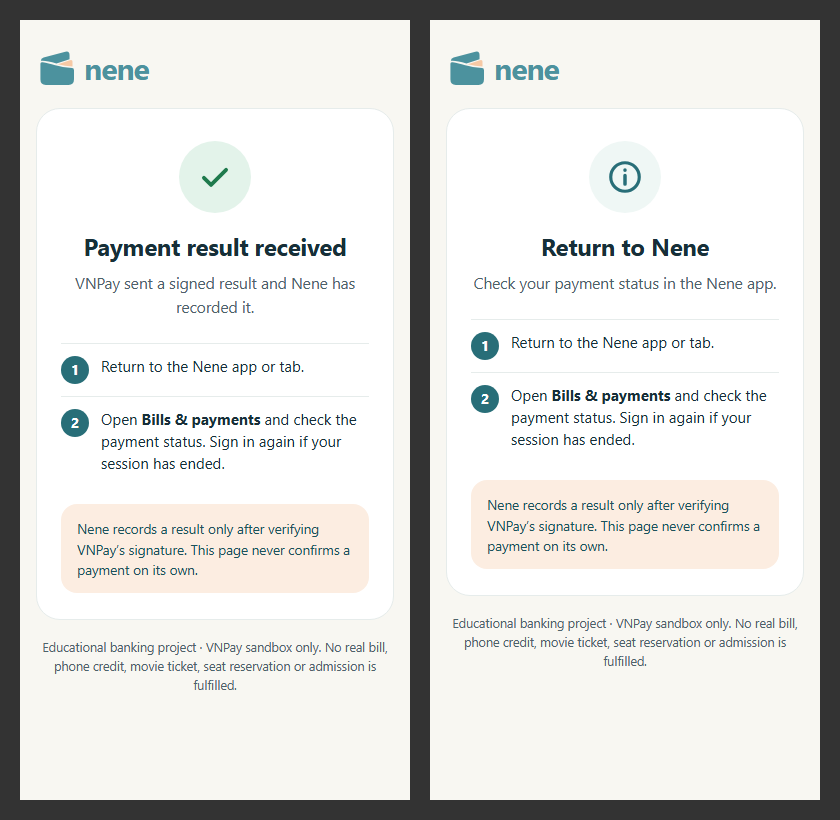
\includegraphics[width=0.75\textwidth]{picture/ch4/vnpay-return-page.png}
\caption{Hai phiên bản của trang quay về từ VNPay sandbox: đã nhận kết quả có chữ ký hợp lệ (trái) và trang mặc định (phải)}
\label{fig:ch4-vnpay-return}
\end{figure}

\section{Nhận xét}
\label{sec:ch4-summary}

Giao diện hiện bao phủ mọi chức năng đã triển khai cho cả hai vai trò, với cùng một hệ thống màu, kiểu chữ, thành phần và cách thể hiện trạng thái. Những điểm còn hạn chế và cần nói rõ:
\begin{itemize}
  \item Ảnh trong chương được dựng từ kiểm thử widget với dữ liệu tổng hợp; kiểm thử đầu--cuối trên điện thoại Android thật vẫn đang tiến hành, và chưa có ảnh của bước kiểm tra khuôn mặt trên thiết bị.
  \item Giao diện mới có tiếng Anh; trợ lý hội thoại hiểu câu hỏi tiếng Việt nhưng trả lời bằng tiếng Anh.
  \item Các chức năng liên ngân hàng, nạp/rút tiền, hóa đơn, nạp điện thoại và vé xem phim đều là mô phỏng hoặc dùng VNPay sandbox, và giao diện ghi rõ điều này trên từng màn hình.
  \item Xác minh khuôn mặt cho giao dịch giá trị cao chưa có; giao diện chặn số tiền từ 5.000.000~VND trở lên thay cho bước này.
\end{itemize}
